\documentclass[12pt]{handout}

\author{Jim Fowler}
\course{Math 1181H}
\date{Autumn 2012}

\usepackage{nopageno}
\usepackage{tikz}
\usepackage{amsmath}

\usetikzlibrary{calc}
\usetikzlibrary{through,positioning}
\usetikzlibrary{arrows}

\DeclareMathOperator{\CAT}{CAT}

\setlength{\parskip}{1.5ex}
\setlength{\parindent}{0in}
\geometry{margin=0.5in}
\usetikzlibrary{patterns}

\title{Isoperimetric inequality}

\begin{document}
\maketitle

How does perimeter compare to enclosed area?  Here are familiar
Euclidean examples.

\begin{center}
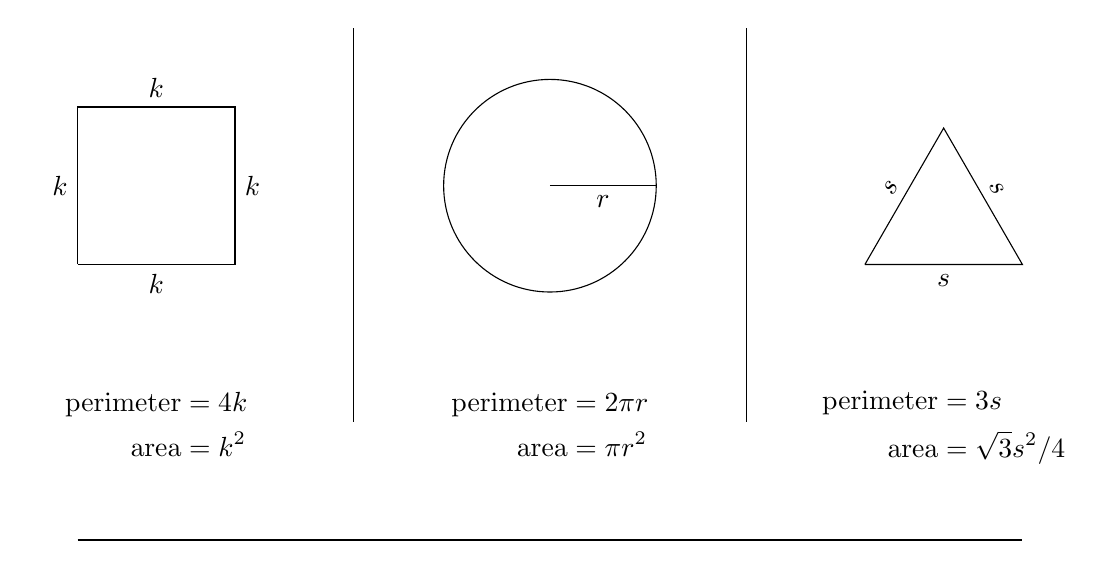
\begin{tikzpicture}
  \draw (0,0) -- (0,2) -- (2,2) -- (2,0) -- (0,0);
  \node[anchor=east] (label1) at (0,1) {$k$};
  \node[anchor=north] (label2) at (1,0) {$k$};
  \node[anchor=west] (label3) at (2,1) {$k$};
  \node[anchor=south] (label4) at (1,2) {$k$};

  \node[anchor=center] (perimeter) at (1,-2) {\parbox{0.25\textwidth}{\begin{align*}
        \mbox{perimeter} &= 4k \\ \mbox{area} &= k^2 %\\ \mbox{a/p} &= k/4 
\end{align*}}};

  \draw (3.5cm,-2) -- (3.5cm,3);
  \draw (8.5cm,-2) -- (8.5cm,3);
  \draw (0cm,-3.5) -- (12cm,-3.5);

  \begin{scope}[xshift=6cm]
  \draw (0,1) circle (1.35);
  \draw (0,1) -- (1.35,1);
  \node[anchor=north] (label4) at (0.5*1.35,1) {$r$};

  \node[anchor=center] (perimeter) at (0,-2) {\parbox[t]{0.25\textwidth}{\begin{align*}
        \mbox{perimeter} &= 2 \pi r  \\ \mbox{area} &= \pi r^2 % \\ \mbox{a/p} &= r / 2
\end{align*}}};
  \end{scope}

  \begin{scope}[xshift=10cm,scale=2]
  \coordinate (a) at (0,0);
  \coordinate (b) at (1,0);
  \coordinate (c) at (0.5,.8660254037);

  \draw (a) -- (b) -- (c) -- (a);
  \node[anchor=north,rotate=0] (label1) at  ($ (a)!0.5!(b) $) {$s$};
  \node[anchor=south,rotate=300] (label2) at  ($ (b)!0.5!(c) $) {$s$};
  \node[anchor=south,rotate=60] (label3) at  ($ (c)!0.5!(a) $) {$s$};

  \node[anchor=center] (perimeter) at (0.5,-1) {\parbox[t]{0.25\textwidth}{\begin{align*}
        \mbox{perimeter} &= 3s  \\ \mbox{area} &= \sqrt{3} s^2 / 4 %\\
                                %\mbox{a/p} &= 3 \sqrt{3} s / 4
\end{align*}}};
  \end{scope}
\end{tikzpicture}
\end{center}

\vfill

\textbf{For a given length, how large an area can we enclose?}  We can
ask this question in a combinatorial setting: the ``curve'' must
follow the edges of the graph paper, and each square in the graph
paper is a unit square.

\begin{center}
  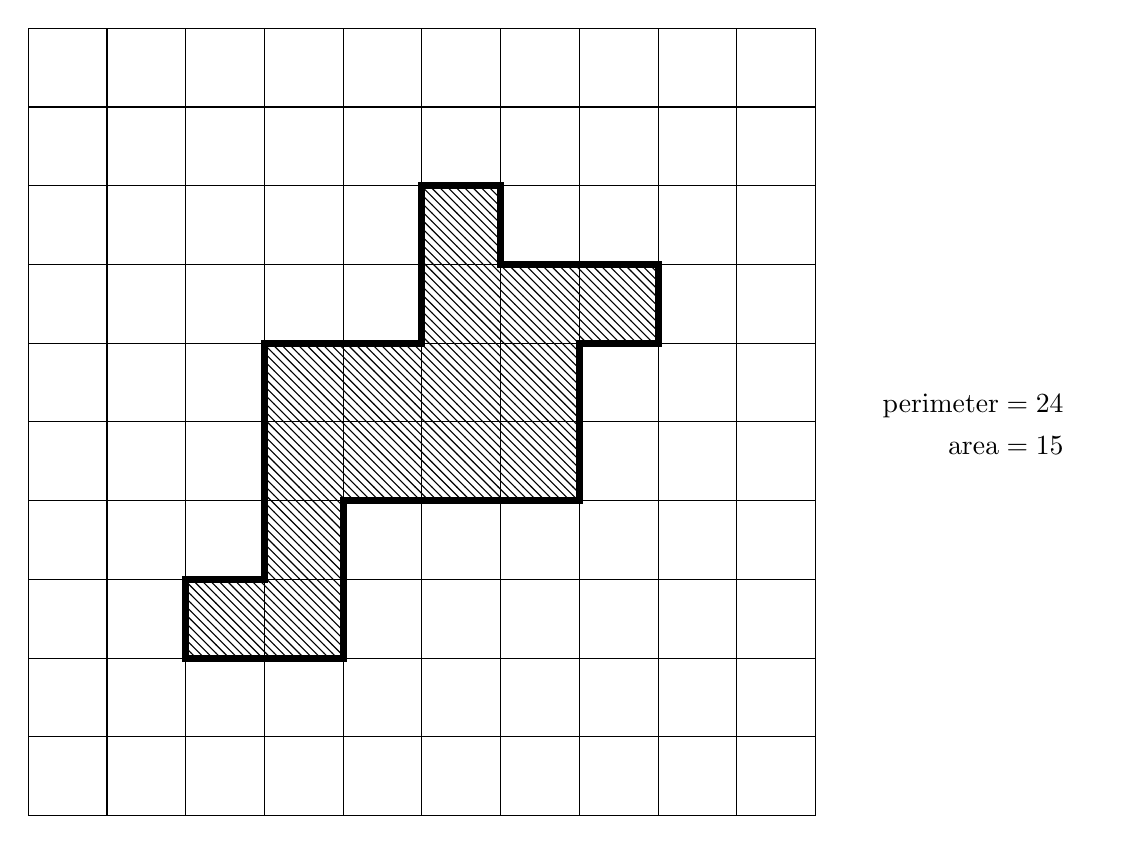
\begin{tikzpicture}
    \foreach \x in {0,...,10}
    \draw (0,\x) -- (10,\x);
    \foreach \x in {0,...,10}
    \draw (\x,0) -- (\x,10);

    \draw[line width=2.5pt] (2,2)
    -- ++(1,0)
    -- ++(1,0)
    -- ++(0,1)
    -- ++(0,1)
    -- ++(1,0)
    -- ++(1,0)
    -- ++(1,0)
    -- ++(0,1)
    -- ++(0,1)
    -- ++(1,0)
    -- ++(0,1)
    -- ++(-1,0)
    -- ++(-1,0)
    -- ++(0,1)
    -- ++(-1,0)
    -- ++(0,-1)
    -- ++(0,-1)
    -- ++(-1,0)
    -- ++(-1,0)
    -- ++(0,-1)
    -- ++(0,-1)
    -- ++(0,-1)
    -- ++(-1,0)
    -- ++(0,-1)
    -- cycle;

    \begin{scope}
    \clip (2,2)
    -- ++(1,0)
    -- ++(1,0)
    -- ++(0,1)
    -- ++(0,1)
    -- ++(1,0)
    -- ++(1,0)
    -- ++(1,0)
    -- ++(0,1)
    -- ++(0,1)
    -- ++(1,0)
    -- ++(0,1)
    -- ++(-1,0)
    -- ++(-1,0)
    -- ++(0,1)
    -- ++(-1,0)
    -- ++(0,-1)
    -- ++(0,-1)
    -- ++(-1,0)
    -- ++(-1,0)
    -- ++(0,-1)
    -- ++(0,-1)
    -- ++(0,-1)
    -- ++(-1,0)
    -- ++(0,-1)
    -- cycle;
    
    \pattern [pattern=north west lines,pattern color=black]
    (0,0) rectangle (10,10);
    \end{scope}

    \node[anchor=center] (description) at (12,5) {\parbox[t]{0.25\textwidth}{\begin{align*}
          \mbox{perimeter} &= 24  \\ \mbox{area} &= 15 \end{align*}}};

  \end{tikzpicture}
\end{center}

\textbf{Can you do better?}  Yes, you can.  There is space on the back
for you to try.

\vfill

\pagebreak

\vfill
\begin{center}
  
\begin{tikzpicture}
    \foreach \x in {0,...,18}
    \draw (0,\x) -- (18,\x);
    \foreach \x in {0,...,18}
    \draw (\x,0) -- (\x,18);
  \end{tikzpicture}
\end{center}
\vfill

\large
\begin{center}
\begin{tabular}{|l|l|}
  \hline
  length of ``curve'' & maximum enclosed area \\
  \hline & \\
  \hline & \\
  \hline & \\
  \hline & \\
  \hline & \\
  \hline & \\
  \hline & \\
  \hline & \\
  \hline & \\
  \hline
\end{tabular}
\hfill
\parbox{0.25\textwidth}{\normalsize \textbf{Definition.} \\ The Dehn function $D(n) = $ the maximum area
  enclosed by a ``curve'' of length $n$.}
\hfill
\null
\end{center}

\vfill

%What happens in $M_5$?
%\begin{center}
%\includegraphics[width=0.8\textwidth]{graphics/plane-5.pdf}
%\end{center}

\end{document}

%%% Local Variables: 
%%% mode: latex
%%% TeX-master: t
%%% End: 
